\documentclass[10pt,a4paper]{article}
\usepackage[utf8]{inputenc}
\usepackage[T1]{fontenc}
\usepackage{listings}
\usepackage[english]{babel}
\usepackage{graphicx}
\usepackage[english]{isodate}
\usepackage[parfill]{parskip}
\usepackage{booktabs}
\usepackage{enumitem}
\usepackage[scaled=0.85]{beramono}


\usepackage{xcolor}

\colorlet{punct}{red!60!black}
\definecolor{background}{HTML}{EEEEEE}
\definecolor{delim}{RGB}{20,105,176}
\colorlet{numb}{magenta!60!black}

\lstdefinelanguage{json}{
    basicstyle=\scriptsize\ttfamily,
    numbers=left,
    numberstyle=\scriptsize,
    stepnumber=1,
    numbersep=8pt,
    showstringspaces=false,
    breaklines=true,
    frame=lines,
    backgroundcolor=\color{background},
    literate=
     *{0}{{{\color{numb}0}}}{1}
      {1}{{{\color{numb}1}}}{1}
      {2}{{{\color{numb}2}}}{1}
      {3}{{{\color{numb}3}}}{1}
      {4}{{{\color{numb}4}}}{1}
      {5}{{{\color{numb}5}}}{1}
      {6}{{{\color{numb}6}}}{1}
      {7}{{{\color{numb}7}}}{1}
      {8}{{{\color{numb}8}}}{1}
      {9}{{{\color{numb}9}}}{1}
      {:}{{{\color{punct}{:}}}}{1}
      {,}{{{\color{punct}{,}}}}{1}
      {\{}{{{\color{delim}{\{}}}}{1}
      {\}}{{{\color{delim}{\}}}}}{1}
      {[}{{{\color{delim}{[}}}}{1}
      {]}{{{\color{delim}{]}}}}{1},
}

\lstdefinelanguage{bash}{
    basicstyle=\normalfont\ttfamily,
    numbers=left,
    numberstyle=\scriptsize,
    stepnumber=10,
    numbersep=8pt,
    showstringspaces=false,
    breaklines=true,
    frame=lines,
    backgroundcolor=\color{background},
    literate=
     *{0}{{{\color{numb}0}}}{1}
      {1}{{{\color{numb}1}}}{1}
      {2}{{{\color{numb}2}}}{1}
      {3}{{{\color{numb}3}}}{1}
      {4}{{{\color{numb}4}}}{1}
      {5}{{{\color{numb}5}}}{1}
      {6}{{{\color{numb}6}}}{1}
      {7}{{{\color{numb}7}}}{1}
      {8}{{{\color{numb}8}}}{1}
      {9}{{{\color{numb}9}}}{1}
      {:}{{{\color{punct}{:}}}}{1}
      {,}{{{\color{punct}{,}}}}{1}
      {\{}{{{\color{delim}{\{}}}}{1}
      {\}}{{{\color{delim}{\}}}}}{1}
      {[}{{{\color{delim}{[}}}}{1}
      {]}{{{\color{delim}{]}}}}{1},
}

\title{TransitMapper Documentation \\ \large{\textbf{Draft}}}
\author{Patrick Brosi}

\begin{document}
\maketitle

\section{Basic Usage}

The input file is a graph given as a (simplified) Geo-JSON file, consisting of nodes (represented as ``Point''-features) and edges (represented as ``LineString''-features). Each edge has a collection of unique ``lines'' that travel through it. The transitmapper will render these lines in a way that resembles a transit map. The input is read from \texttt{stdin}.


\begin{lstlisting}[language=bash,firstnumber=1]
$ transitmapper -o test.svg < test.json
\end{lstlisting}

See below for an example input.

\begin{figure}[htbp]
  \centering
$	\vcenter{\hbox{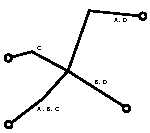
\includegraphics[width=0.33\textwidth]{inputex.pdf}}}$
	\hspace{5mm}
	$	\vcenter{\hbox{\scalebox{2}{\large $\Rightarrow$}}} $
	\hspace{5mm}
$	\vcenter{\hbox{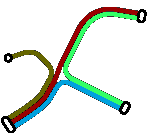
\includegraphics[width=0.33\textwidth]{test2.pdf}}}$
  \caption{Simple example output}
\end{figure}

\section{Command line parameters}

The following command line parameters are accepted by \texttt{transitmapper} (see also \texttt{-{}-help}).

\begin{description}[align=right]
	\item[\texttt{-{}-line-width=N}] The default width of a line, in output units. 20 by default.
	\item[\texttt{-{}-line-spacing=N}] The default spacing between lines, in output units. 10 by default.
	\item[\texttt{-{}-render-station-names}] Output the station names (experimental).
	\item[\texttt{-{}-render-node-fronts}] Output node fronts, useful for debugging.
	\item[\texttt{-{}-resolution=D}] Output resolution. 0.1 by default.
	\item[\texttt{-{}-no-optim}] (\texttt{-N}) Disable line-ordering optimization.
	\item[\texttt{-{}-input-smoothing=D}] Level of input-data smoothing. 3 by default.
\end{description}

\begin{figure}
  \centering
	$	\vcenter{\hbox{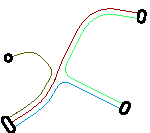
\includegraphics[width=0.33\textwidth]{test2_thin.pdf}}}$
	\hspace{5mm}
$	\vcenter{\hbox{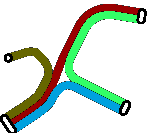
\includegraphics[width=0.33\textwidth]{test2_thick.pdf}}}$
	\caption{Different settings of \texttt{-{}-line-width} and \texttt{-{}-line-spacing}}
\end{figure}

\begin{figure}
  \centering
$	\vcenter{\hbox{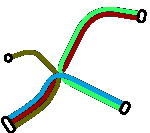
\includegraphics[width=0.33\textwidth]{test2_noopt.pdf}}}$
	\caption{Output without ordering optimization (\texttt{-N})}
\end{figure}

\begin{figure}
  \centering
$	\vcenter{\hbox{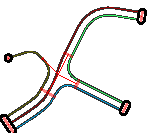
\includegraphics[width=0.33\textwidth]{test2_nodefronts.pdf}}}$
	\caption{Node-front rendering (\texttt{-{}-render-node-fronts})}
\end{figure}

\begin{figure}
  \centering
$	\vcenter{\hbox{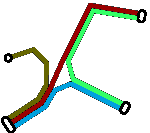
\includegraphics[width=0.33\textwidth]{test2_nosmoothing.pdf}}}$
	\caption{Without any line smoothing (\texttt{-{}-input-smoothing=0 -{}-bezier-prec=0})}
\end{figure}

\section{JSON Format}

See also ??. The input format is a lightweight subset of GeoJSON. At the top level, the input JSON must contain a \texttt{FeatureCollection} object:


\begin{lstlisting}[language=json,firstnumber=1]
{
  "type": "FeatureCollection",
  "features": [...]
}
\end{lstlisting}

A \texttt{feature} can either be a node (a \texttt{point}) or an edge (a \texttt{LineString}).

\subsection{Nodes}

A node consists of a geometry (the node's coordinates) and some properties.

\begin{lstlisting}[language=json,firstnumber=1]
{
  "geometry": {
	"coordinates": [0, 0],
	"type": "Point"
  },
  "properties": {
	"id": "1",
	"station_id": "1"
  }
}
\end{lstlisting}

\texttt{Type} is always \texttt{"point"}. The \texttt{coordinates} are given as an \texttt{[x,y]} array.

\subsubsection{Node Properties}

\begin{description}[align=right]
  \item[\texttt{id}] A dataset-unique string identifier for this node. Will be referenced later in edges.
  \item[\texttt{station\_id}] If this node is a station, the station's unique id (optional).
  \item[\texttt{station\_label}] If this node is a station, the station's name (optional). Either \texttt{station\_id} or \texttt{station\_label} has to be set for a node to become a station.
  \item[\texttt{excluded\_line\_connections}] A list of lines that are not connected in this node, even though two or more edges containing the line start/end in the node. The \texttt{line\_id} (see ??) as well as the two edges this line is not connected in has to be given. Both edges are identified by the adjacent node. Example:
\begin{lstlisting}[language=json,firstnumber=1]
"excluded_line_connections": [
  {
	"edge1_node": "2",
	"edge2_node": "3",
	"route": "A"
  },
  {
	"edge1_node": "4",
	"edge2_node": "6",
	"route": "B"
  }
]
\end{lstlisting}

\begin{figure}
  \centering
$	\vcenter{\hbox{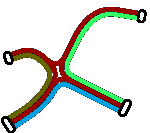
\includegraphics[width=0.33\textwidth]{test3.pdf}}}$
	\caption{The red line is not connected between the two main axes (via \texttt{exluded\_line\_connections})}
\end{figure}

\end{description}

\subsection{Edges}

An edge consists also of a geometry (a linestring) and some properties.

\begin{lstlisting}[language=json,firstnumber=1]
{
  "geometry": {
	"coordinates": [
	  [0, 0], [500, 900], [1000, 950]
	],
	"type": "LineString"
  },
  "properties": {
	"from": "1",
	"to": "2",
	"lines": [
	  {"color": "00a1de"},
	  {"color": "990000"}
	]
  }
}
\end{lstlisting}

Properties \texttt{from} and \texttt{to} hold the IDs of the nodes this edges connects. 

\begin{description}[align=right]
  \item[\texttt{id}] A dataset-unique string identifier for this node. Will be referenced later in edges.

\end{description}

\begin{figure}
  \centering
$	\vcenter{\hbox{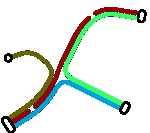
\includegraphics[width=0.33\textwidth]{test4.pdf}}}$
	\caption{Directed line occurances (via \texttt{direction})}
\end{figure}

\begin{figure}
  \centering
$	\vcenter{\hbox{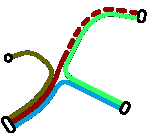
\includegraphics[width=0.33\textwidth]{test_dashed.pdf}}}$
	\caption{Dashed line (via \texttt{"dash-array"="4 2"})}
\end{figure}

\section{Example Input}


\begin{lstlisting}[language=json,firstnumber=1]
{
  "type": "FeatureCollection",
  "features": [
    {
      "geometry": {
        "coordinates": [0, 0],
        "type": "Point"
      },
      "properties": {
        "id": "1",
        "station_id": "1"
      }
    },
    {
      "geometry": {
        "coordinates": [1000, 1000],
        "type": "Point"
      },
      "properties": {
        "id": "2",
        "station_id": "2"
      },
      "type": "Feature"
    },
    {
      "geometry": {
        "coordinates": [
          [0, 0], [500, 900], [1000, 950]
        ],
        "type": "LineString"
      },
      "properties": {
        "from": "1",
        "to": "2",
        "lines": [
          {"color": "00a1de"},
          {"color": "990000"}
        ]
      }
    }
  ]
}
\end{lstlisting}
\end{document}
